\section{Sampling Metodları}
Veri analizi ve makine öğrenimi projelerinde, dengesiz veri setleri sıkça karşılaşılan bir sorundur. Özellikle sınıflandırma problemlerinde, nadir sınıfların fazla sınıflara göre daha az örneklenmiş olması, modelin yanlış sonuçlar üretmesine neden olabilir. İşte bu durumda, oversampling ve undersampling gibi teknikler devreye girer.

Oversampling, nadir sınıflara ait örnekleri çoğaltarak veya yeniden örnekleme yaparak veri setinin dengesini sağlama işlemidir. Bu yöntem, nadir sınıfların temsil edilme oranını artırarak modelin daha dengeli bir şekilde eğitilmesini sağlar. Undersampling, fazla sınıflara ait örnekleri azaltarak veya örnekleri rastgele seçerek veri setinin dengesini sağlama işlemidir. Bu yöntem, fazla sınıfların temsil edilme oranını azaltarak veri setini daha dengeli hale getirir. Undersampling, modelin dengeli bir şekilde eğitilmesini sağlayabilir, ancak nadir sınıfların temsil edilme oranını azaltma riski taşır.

\begin{itemize}
    \item Dengesiz sınıf dağılımı düşük tespit oranına (recall score) yol açar.
    \item Örneklem arttırma (oversampling), örneklem azaltma (undersampling)
    \item Çoğunluk (majority), azınlık (minority)
\end{itemize}

Under Sampling Metodları
\begin{enumerate}
    \item Dönüştürülmüş Veri Seti Üzerinden Örneklem Seçen Metodlar
    \begin{enumerate}
        \item \textbf{Near Miss Undersampling:} Çoğunluk sınıfın azınlık sınıflara uzaklığına göre bu örneklemleri seçen bir örneklem azaltma metodudur.
        \item \textbf{Condensed Nearest Neighbors Rule:} CNN, KNN algoritmasının memory ihtiyacını azaltması için üretildi.
    \end{enumerate}
    \item Silinecek Örnekleri Seçen Metodlar
    \begin{enumerate}
        \item \textbf{Tomek Links:} Her bir sınıftan en yakın Öklid uzaklığına sahip birer tane örnek ile pair (çift) duruma gelmesini kural olarak koyar ve bu sınıflar arası oluşan çiftler Tomek linkler olarak adlandırılır.
        \item \textbf{Edited Nearest Neighbors Rule:} Kısa adı ENN. Veri setindeki belirsiz, gürültülü örnekleri ortadan kaldırmak için kullanılır. Veriden mümkün olduğunda az bilgi kaybına yol açarak yoğunluk sınıfını azaltması sağladığı en büyük faydadır.
    \end{enumerate}
    \item Hibrit Metodlar
    \begin{enumerate}
        \item \textbf{One Sided Selection:} Kısa adı OSS. Tomek Link ve CNN rule metodlarını kombinleyen bir metoddur. Tomek linklerinin sınırda ve gürültülü tüm veri örneklerini kaldırmasıyla oluşturduğu alt kümenin ardından CNN karar sınıfından uzaktaki çoğunluk sınıfı örneklerini veri setinden kaldırır.
        \item \textbf{Neighborhood Cleaning Rule:} CNN ve ENN metodlarını kombinleyen bir metoddur.
    \end{enumerate}
\end{enumerate}

Over Sampling Metodları

\begin{enumerate}
    \item Rastgele Oversampling
    \begin{enumerate}
        \item \textbf{Rastgele Tekrarlı Örnekleme (Random Oversampling):} Azınlık sınıftaki örnekleri rastgele seçerek artırır.
        \item \textbf{Rastgele SMOTE (Random SMOTE):} SMOTE yöntemini temel alır ve sentetik örnekler oluşturur, ancak bu işlemde rastgele seçilen örnekler kullanılır.
    \end{enumerate}
    \item Sentetik Oversampling
    \begin{enumerate}
        \item \textbf{SMOTE:} Azınlık sınıfındaki örnekleri kullanarak sentetik örnekler oluşturur.
        \item \textbf{ADASYN (Adaptive Synthetic Sampling):} Örneklerin yoğunluğuna göre sentetik örnekler üretir, özellikle azınlık sınıfındaki zor örnekler üzerinde odaklanır.
        \item \textbf{Borderline-SMOTE:} Sınıf sınırında yer alan örnekler üzerine odaklanır ve sentetik örnekler bu sınıflarda oluşturulur.
    \end{enumerate}
\end{enumerate}

\newpage

\subsection{Oversampling}

\subsubsection{SMOTE (Synthetic Minority Over-Sampling Technique)}
Azınlık sınıfındaki her bir örneğe rastgele seçilen komşuları arasında bir veya birkaç benzer örnek oluşturur. Bu benzer örnekler arasında yeni sentetik örnekler oluşturulur. Bu, azınlık sınıfın örneklerini birbirine bağlar ve böylece sınıfın veri dağılımını artırır. Veri setini değiştirmez sadece yeni örnekler ekler. Overfitting riskini azaltır. Eğer orjinal veri setindeki örnekler birbirine çok benzeyen verilerse, sentetik verilerin de bu özellikleri yansıtması overfitting riskini artırabilir.

\begin{lstlisting}[language=Python]
from imblearn.over_sampling import SMOTE

sm = SMOTE(random_state=42)
X_resampled, y_resampled = sm.fit_resample(X_train, y_train)
\end{lstlisting}

\begin{figure}[h]
    \centering
    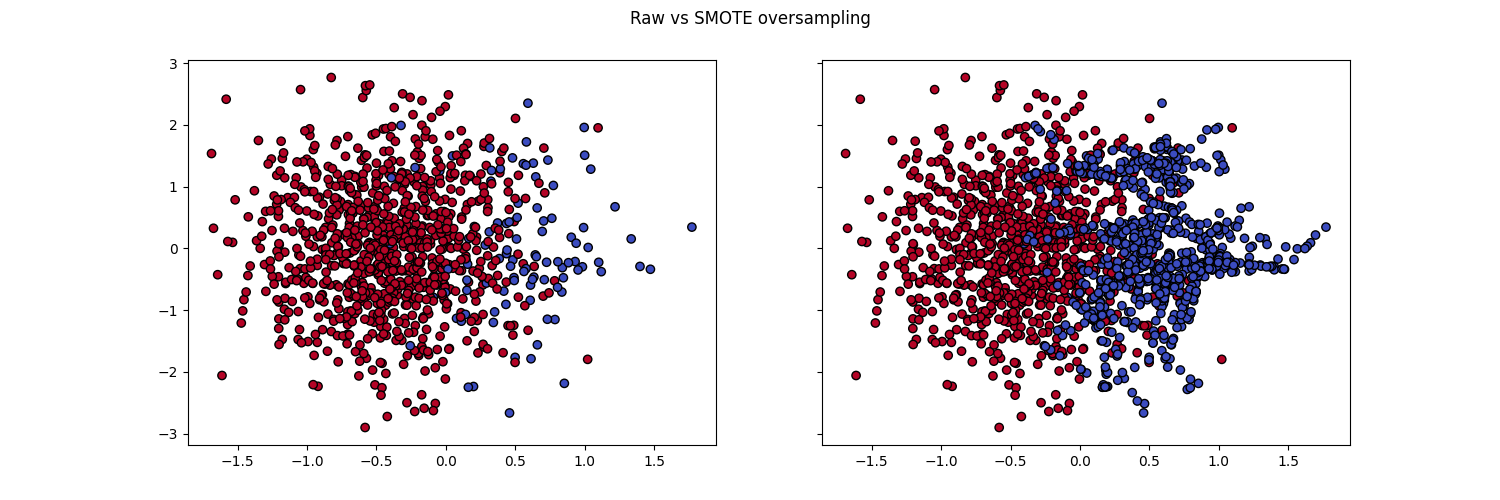
\includegraphics[width=1\textwidth]{images/Raw vs SMOTE oversampling.png}
    \caption{SMOTE örneği.}
    \label{fig:enter-label}
\end{figure}

\newpage

\subsubsection{ADASYN (Adaptive Synthetic Sampling)}
Azınlık sınıfındaki her örneğin etrafındaki hedeflenen komşuluk yoğunluğunu ölçer. Daha az temsil edilen örneklerin etrafında daha fazla sentetik örnek oluşturur. Bu azınlık sınıfındaki daha az temsil edilen bölgelerin daha fazla ağırlığı sahip olmasını sağlar. Sentetik örneklerin daha adaptif bir şekilde oluşturulması, daha az temsil edilen bölgelerde daha fazla vurgu yapılmasına olanak tanır.

\begin{lstlisting}[language=Python]
from imblearn.over_sampling import ADASYN

ada = ADASYN()
X_resampled, y_resampled = ada.fit_resample(X_train, y_train)
\end{lstlisting}

\begin{figure}[h]
    \centering
    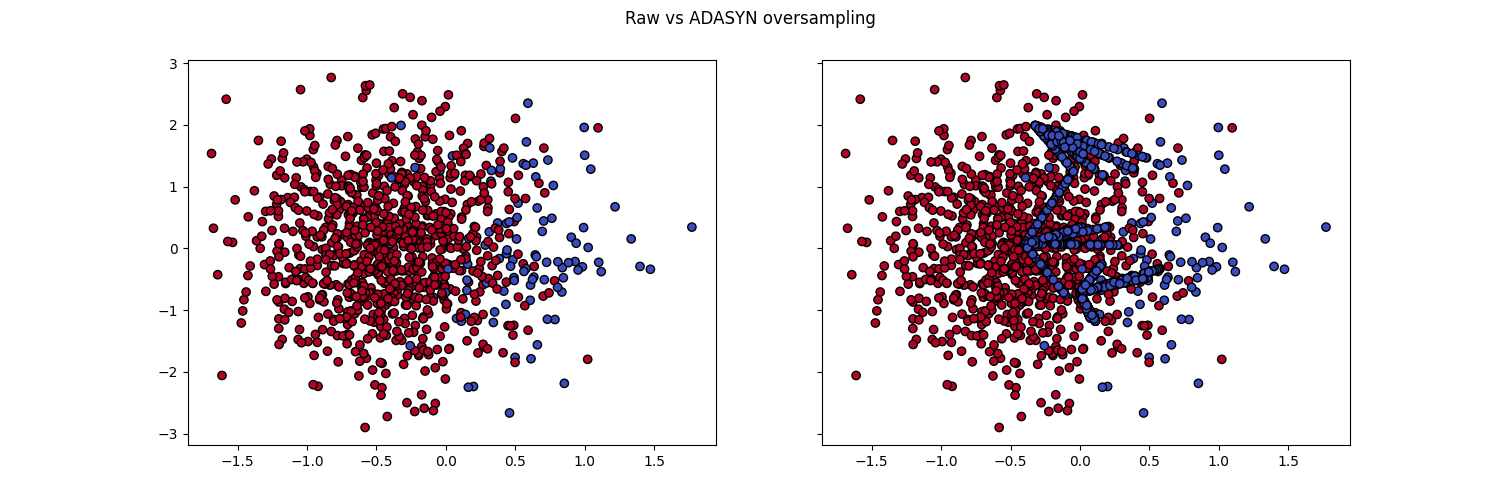
\includegraphics[width=1\textwidth]{images/Raw vs ADASYN oversampling.png}
    \caption{ADASYN örneği.}
    \label{fig:enter-label}
\end{figure}

\newpage

\subsubsection{Borderline-SMOTE}
Azınlık sınıfındaki örnekler arasında, sınıf sınırlarına yakın olanları belirler. Bu örnekler, genellikle çoğunluk sınıfına daha yakın olup karar sınırlarında yer alan veri noktalarıdır. Sınıf sınırındaki bu örnekler üzerinde sentetik örnekler oluşturarak azınlık sınıfının veri dağılımını artırır. Sentetik örnekler, gerçek verilere benzemesi için bu sınırlardaki veri noktalarının arasında oluşturulur.

\begin{lstlisting}[language=Python]
from imblearn.over_sampling import BorderlineSMOTE

bsm = BorderlineSMOTE()
X_resampled, y_resampled = bsm.fit_resample(X_train, y_train)
\end{lstlisting}

\begin{figure}[h]
    \centering
    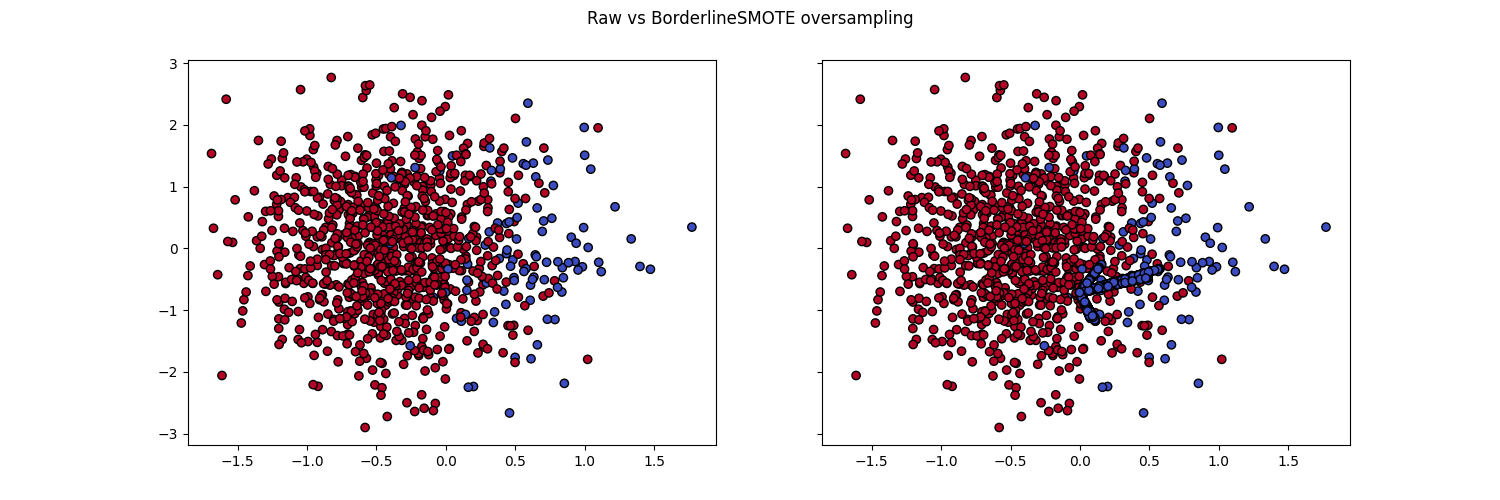
\includegraphics[width=1\textwidth]{images/Raw vs BorderlineSMOTE oversampling.png}
    \caption{Borderline-SMOTE örneği.}
    \label{fig:enter-label}
\end{figure}

\newpage

\subsubsection{Random Over Sampler}
Azınlık sınıfındaki örneklerin sayısına eşit olacak şekilde, çoğunluk sınıfındaki örnekler rastgele seçilerek artırılır. Bu seçilen örnekler, azınlık sınıfındaki mevcut örneklerle birleştirilerek dengeli bir veri seti oluşturulur. Mevcut veri setini değiştirmez sadece örneklerin tekrarlanmasını kullanır.

\begin{figure}[h]
    \centering
    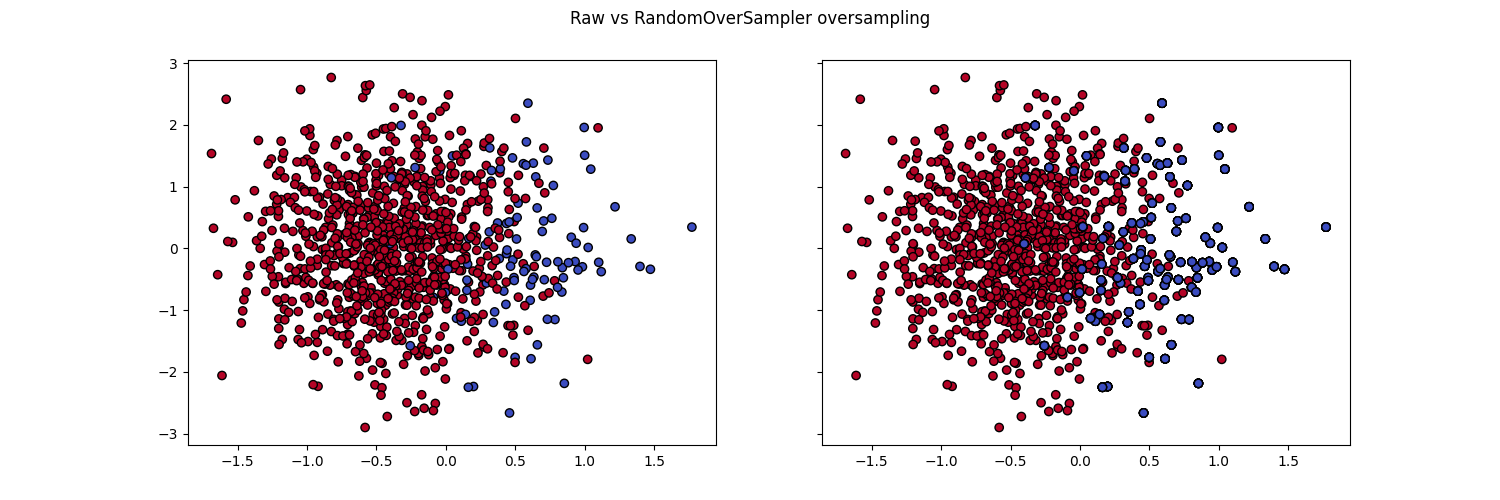
\includegraphics[width=1\textwidth]{images/Raw vs RandomOverSampler oversampling.png}
    \caption{RandomOverSampler örneği.}
    \label{fig:enter-label}
\end{figure}

\begin{lstlisting}[language=Python]
from imblearn.over_sampling import RandomOverSampler

ros = RandomOverSampler(sampling_strategy=1.0, random_state=42)
X_resampled, y_resampled = ros.fit_resample(X_train, y_train)
\end{lstlisting}

\newpage

\subsection{Undersampling}

\subsubsection{ClusterCentroids}
Azınlık sınıfındaki veri noktalarının küme merkezlerini hesaplar. Bu küme merkezleri, çoğunluk sınıfındaki veri noktalarıyla değiştirilir. Bu, azınlık sınıfını temsil etmek için yeni bir alt örneklem oluşturur.

\begin{lstlisting}[language=Python]
from imblearn.under_sampling import ClusterCentroids

cc = ClusterCentroids(random_state=42)
X_resampled, y_resampled = cc.fit_resample(X_train, y_train)
\end{lstlisting}

\begin{figure}[h]
    \centering
    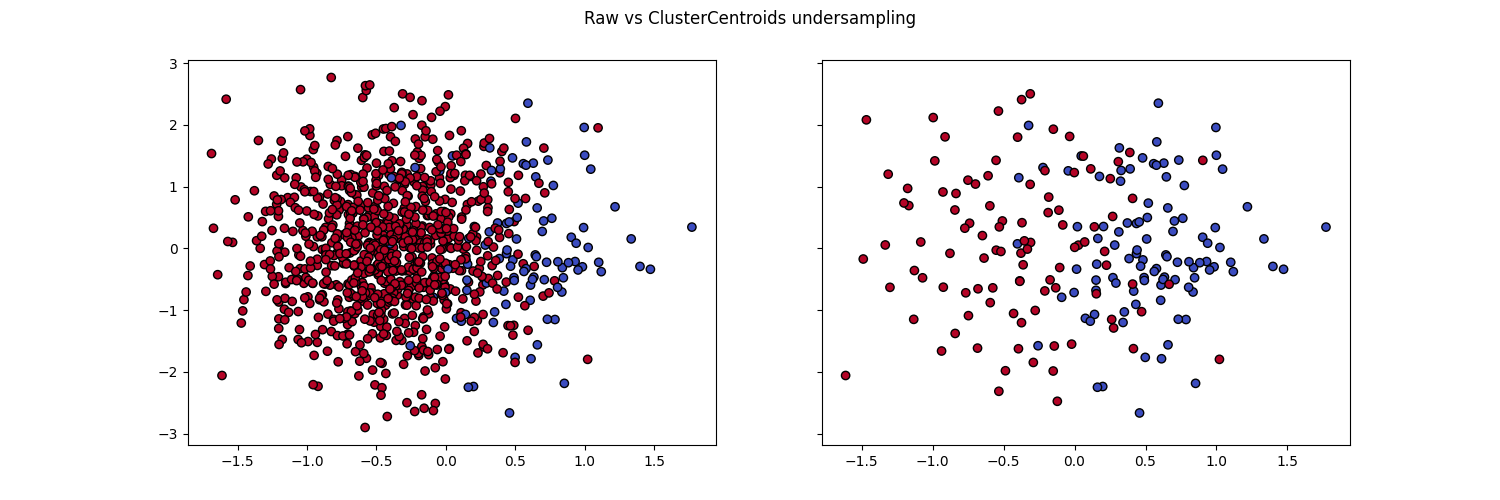
\includegraphics[width=1\textwidth]{images/Raw vs ClusterCentroids undersampling.png}
    \caption{ClusterCentroids örneği.}
    \label{fig:enter-label}
\end{figure}

\newpage

\subsubsection{Random Under Sampler}
Çoğunluk sınıfından rastgele örnekler seçerek, azınlık sınıfındaki örnek sayısıyla aynı sayıya düşürür. Bu seçilen örnekler, çoğunluk sınıfındaki veri sayısını azaltarak daha dengeli bir veri seti oluşturur.

\begin{lstlisting}[language=Python]
from imblearn.under_sampling import RandomUnderSampler

rus = RandomUnderSampler(sampling_strategy=1.0, random_state=42)
X_resampled, y_resampled = rus.fit_resample(X_train, y_train)
\end{lstlisting}

\begin{figure}[h]
    \centering
    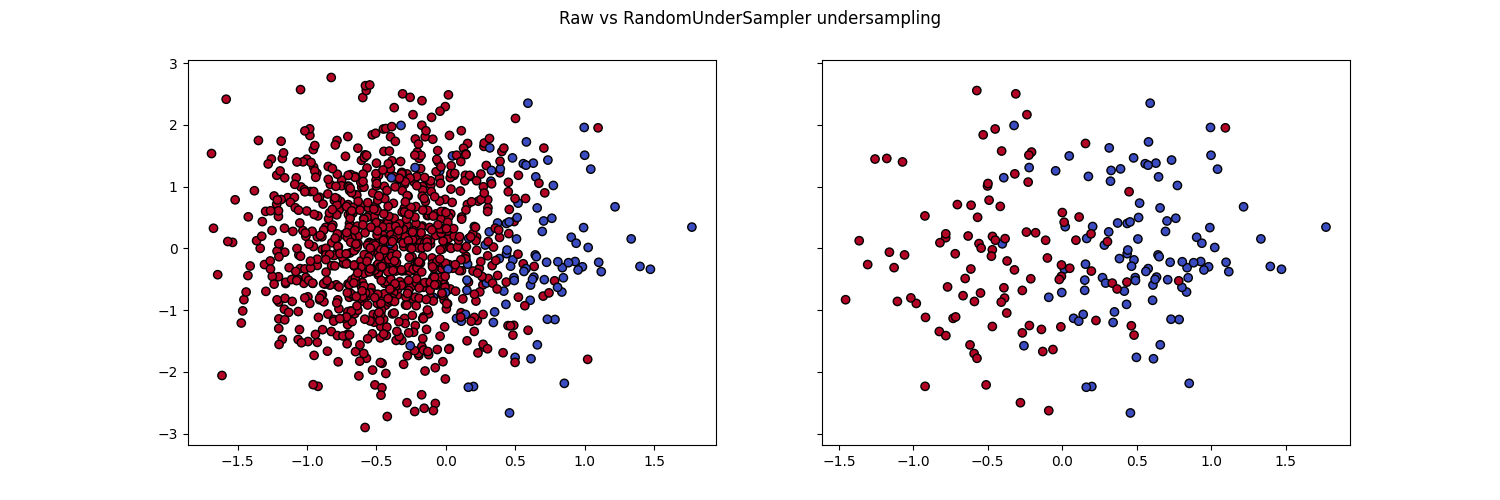
\includegraphics[width=1\textwidth]{images/Raw vs RandomUnderSampler undersampling.png}
    \caption{RandomUnderSampler örneği.}
    \label{fig:enter-label}
\end{figure}

\newpage

\subsubsection{NearMiss}
Azınlık sınıfına daha yakın olan çoğunluk sınıfı örneklerini belirlemek için bir kriter kullanır. Bu kriter, belirli bir eşik değeri veya uzaklık ölçüsüne dayanır. Seçilen çoğunluk sınıfı örnekleri, azınlık sınıfı ile aralarındaki uzaklık veya farklılık kriterini en iyi şekilde karşılayan örneklerdir. Bu örnekler seçilerek alt örnekleme işlemi gerçekleştirilir.

\begin{lstlisting}[language=Python]
from imblearn.under_sampling import NearMiss

nm = NearMiss()
X_resampled, y_resampled = nm.fit_resample(X_train, y_train)
\end{lstlisting}

\begin{figure}[h]
    \centering
    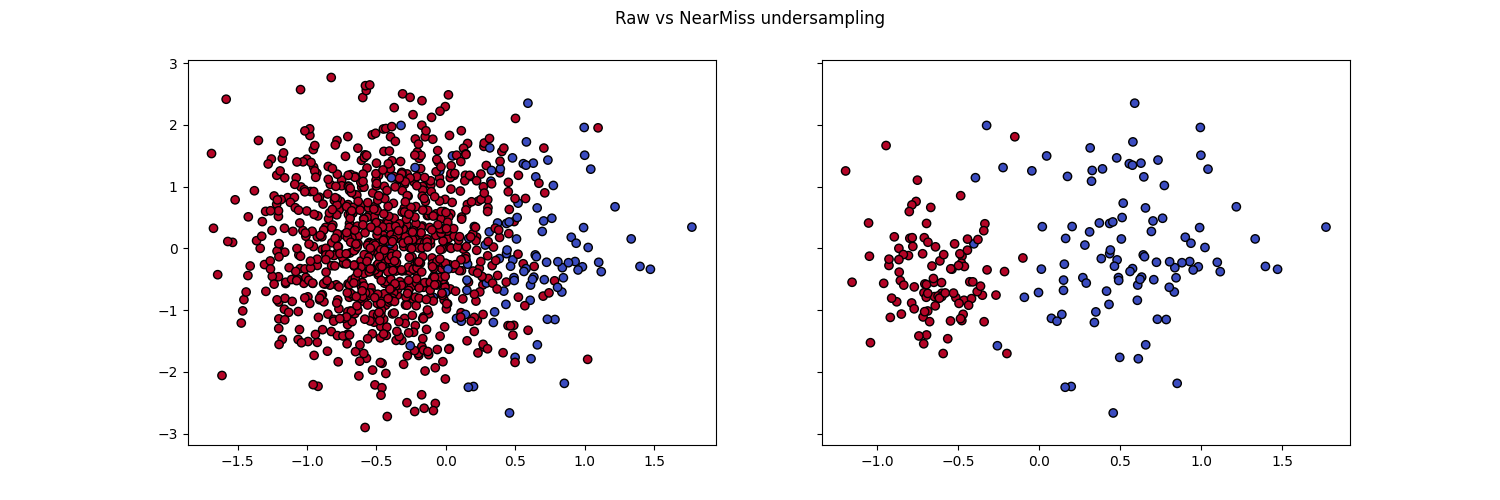
\includegraphics[width=0.8\textwidth]{images/Raw vs NearMiss undersampling.png}
    \caption{NearMiss örneği.}
    \label{fig:enter-label}
\end{figure}

\newpage

\subsubsection{TomekLinks}
Veri setindeki her bir veri noktası için o veri noktasına en yakın komşusunu bulur. Eğer iki veri noktası birbirlerinin en yakın komşusuysa ve aynı sınıfa ait değillerse, bu iki veri noktası arasındaki ilişkiyi (tomek link) belirler. Bu tomek linke sahip olan veri noktalarından çoğunluk sınıfına ait olan çıkararak veri dengesizliğini azaltır.

\begin{lstlisting}[language=Python]
from imblearn.under_sampling import TomekLinks

tomeklinks = TomekLinks(sampling_strategy="auto")
X_resampled, y_resampled = tomeklinks.fit_resample(X_train, y_train)
\end{lstlisting}

\begin{figure}[h]
    \centering
    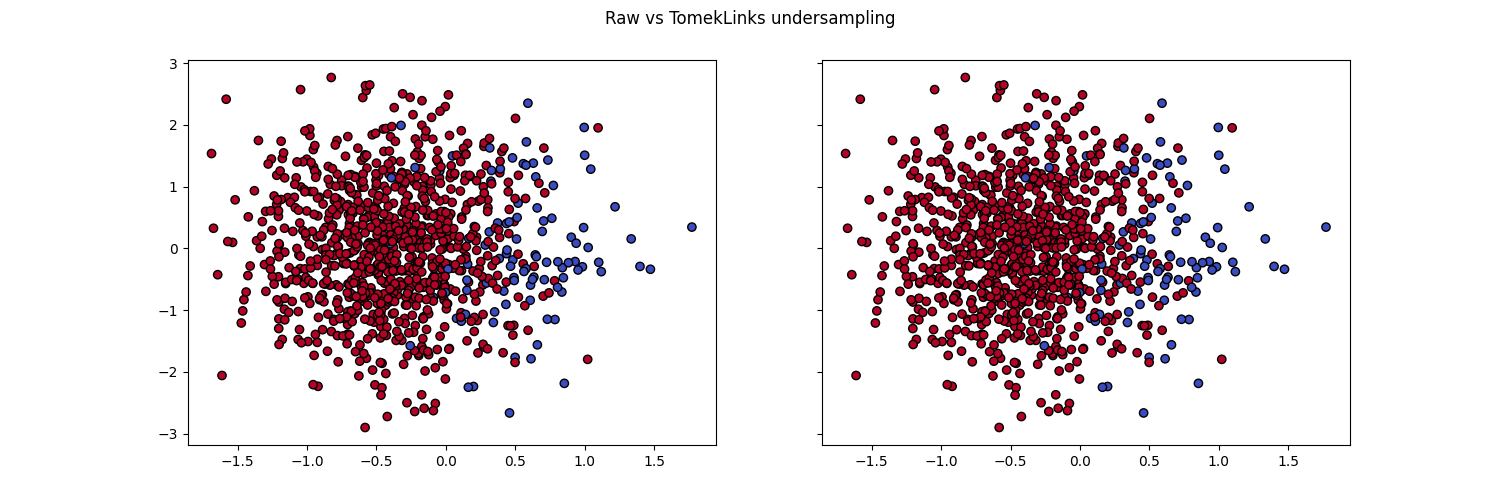
\includegraphics[width=0.8\textwidth]{images/Raw vs TomekLinks undersampling.png}
    \caption{TomekLinks örneği.}
    \label{fig:enter-label}
\end{figure}

\newpage

\subsubsection{CondensedNearestNeighbour}
Veri setindeki bir örnek seçilir. Seçilen bu örnek aynı sınıfa ait komşuları ile karşılaştırılır. Eğer bu örnek, aynı sınıfa ait komşularından farklı bir sınıfa aitse, bu örnek korunur ve yeni alt örnekleme setine eklenir. Diğer tüm örnekler bu kriterlere göre kontrol edilir ve veri setinden aynı bilgiyi koruyarak daha küçük bir alt örnekleme seti oluşturulur.

\begin{lstlisting}[language=Python]
from imblearn.under_sampling import CondensedNearestNeighbour

cnn = CondensedNearestNeighbour(random_state=42)
X_resampled, y_resampled = cnn.fit_resample(X_train, y_train)
\end{lstlisting}

\begin{figure}[h]
    \centering
    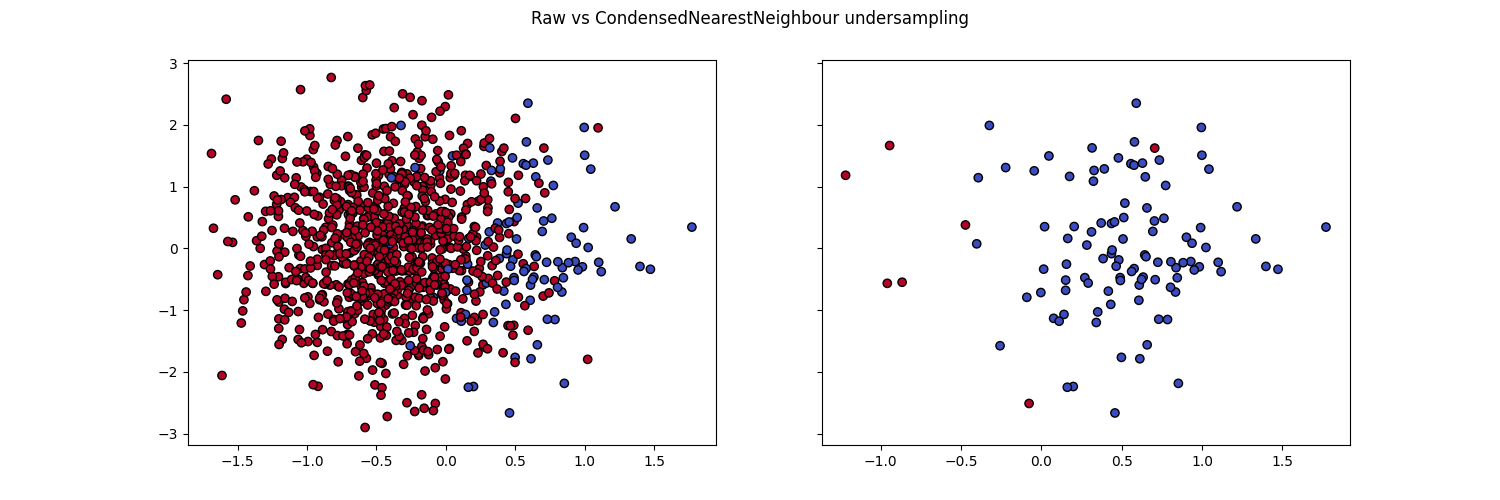
\includegraphics[width=0.8\textwidth]{images/Raw vs CondensedNearestNeighbour undersampling.png}
    \caption{CondensedNearestNeighbour örneği.}
    \label{fig:enter-label}
\end{figure}

\newpage

\subsubsection{OneSidedSelection}
Azınlık sınıfından rastgele bir örnek seçilir. Seçilen bu örnek, çoğunluk sınıfındaki komşuları ile karşılaştırılır. Eğer bu örnek, çoğunluk sınıfındaki örneklerin etkileşimli olduğu bir bölgede bulunmuyorsa ve azınlık sınıfına aitse, bu örnek korunur ve yeni alt örnekleme setine eklenir. Diğer azınlık sınıfı örnekleri de bu şekilde kontrol edilir ve belirli bir kriteri sağlayan örnekler korunarak daha dengeli bir alt örnekleme seti oluşturulur.

\begin{lstlisting}[language=Python]
from imblearn.under_sampling import OneSidedSelection

oss = OneSidedSelection(random_state=0, n_seeds_S=10)
X_resampled, y_resampled = oss.fit_resample(X_train, y_train)
\end{lstlisting}

\begin{figure}[h]
    \centering
    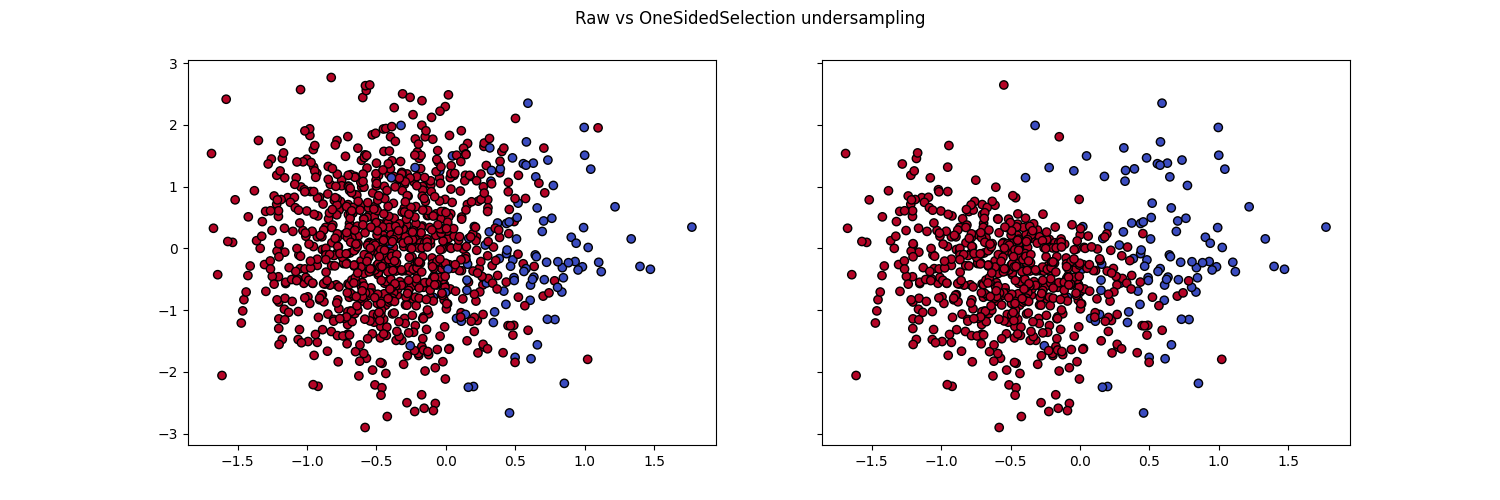
\includegraphics[width=0.8\textwidth]{images/Raw vs OneSidedSelection undersampling.png}
    \caption{OneSidedSelection örneği.}
    \label{fig:enter-label}
\end{figure}

\newpage

\subsubsection{Neighbourhood Cleaning Rule}
Azınlık sınıfındaki bir örnek seçilir. Seçilen bu örnek, çoğunluk ve azınlık sınıflarının sınırlarındaki bölgelerdeki örnekleri inceler. Eğer bir örnek, kendi sınıfına ait değilse veya farklı bir sınıfa ait komşuları varsa, bu örnek kaldırılır. Diğer örnekler de aynı şekilde incelenerek belirli bir kriteri sağlamayan örnekler kaldırılır ve daha dengeli bir alt örnekleme seti oluşturulur.

\begin{lstlisting}[language=Python]
from imblearn.under_sampling import NeighbourhoodCleaningRule

ncr = NeighbourhoodCleaningRule(sampling_strategy="auto", n_neighbors=250, threshold_cleaning=0.5)
X_resampled, y_resampled = ncr.fit_resample(X_train, y_train)
\end{lstlisting}

\begin{figure}[h]
    \centering
    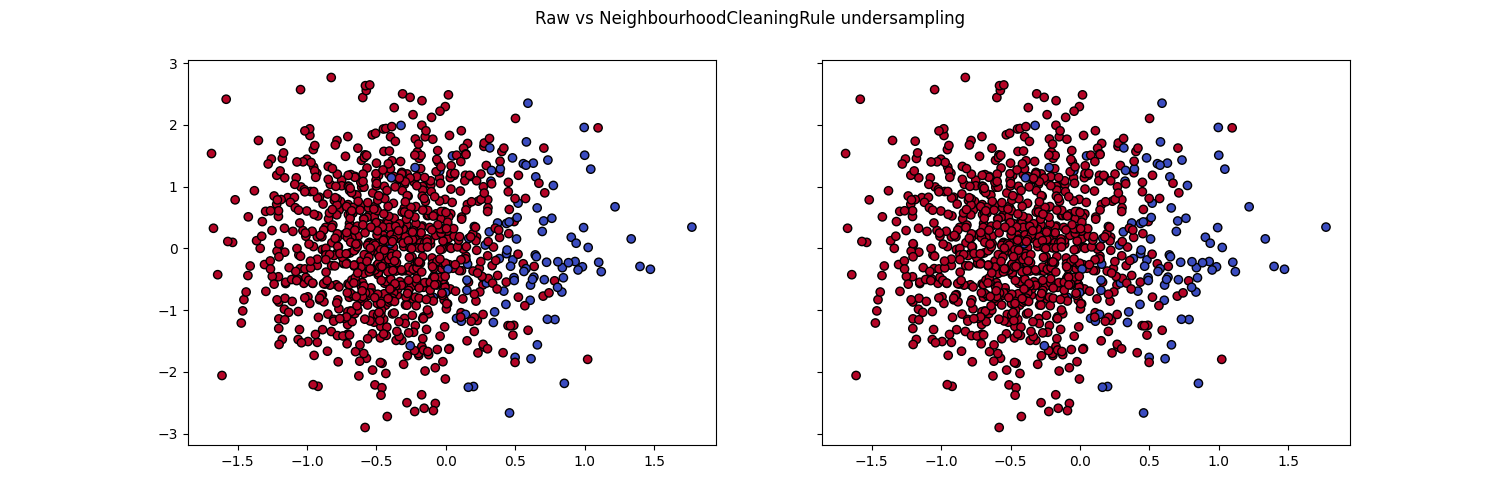
\includegraphics[width=0.6\textwidth]{images/Raw vs NeighbourhoodCleaningRule undersampling.png}
    \caption{NeighbourhoodCleaningRule örneği.}
    \label{fig:enter-label}
\end{figure}

\newpage

\subsubsection{EditedNearestNeighbours (ENN)}
Başlangıçta, veri setindeki her bir örneğin sınıf etiketleri kontrol edilir. Her bir örnek için, bu örneğin sınıf etiketi ile k-NN (k en yakın komşu) algoritması kullanılarak belirlenen komşuların sınıf etiketleri karşılaştırılır. Eğer bir örnek, en azından biriyle komşu olmak üzere çoğunluk sınıfı etiketine sahip bir komşusu varsa ve kendisi azınlık sınıfına aitse, bu örnek veri setinden çıkarılır. Diğer örnekler de aynı şekilde incelenerek belirli bir kriteri sağlamayan örnekler kaldırılır ve daha dengeli bir alt örnekleme seti oluşturulur.

\begin{lstlisting}[language=Python]
from imblearn.under_sampling import EditedNearestNeighbours

enn = EditedNearestNeighbours(sampling_strategy='auto', n_neighbours=300, kind_sel='all')
X_resampled, y_resampled = enn.fit_resample(X_train, y_train)
\end{lstlisting}

\begin{figure}[h]
    \centering
    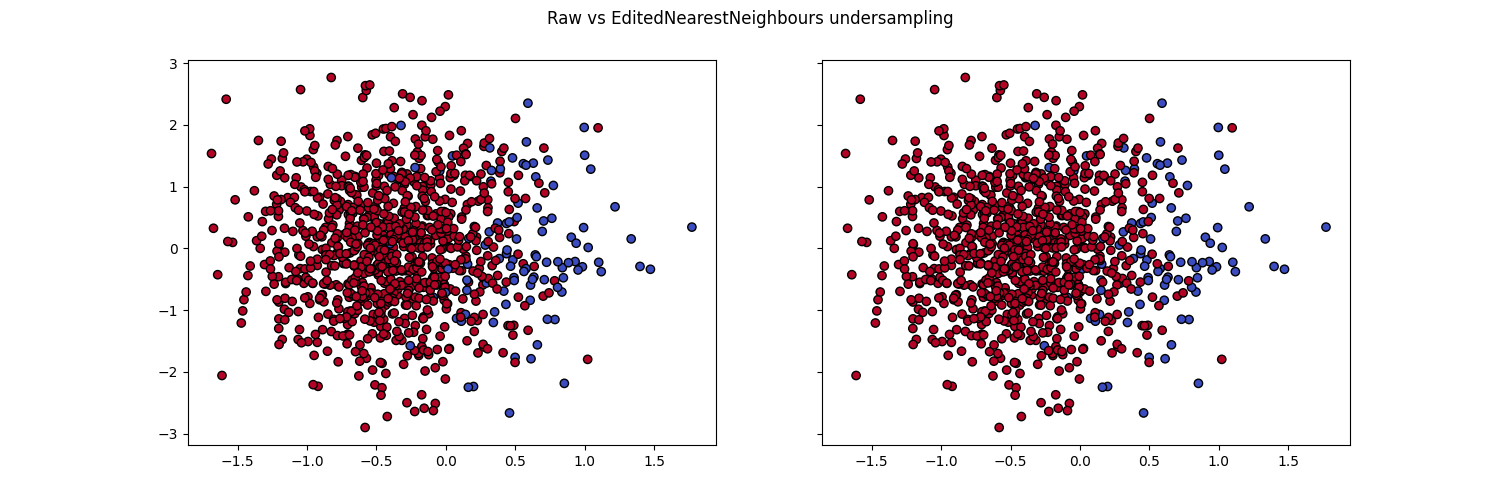
\includegraphics[width=0.6\textwidth]{images/Raw vs EditedNearestNeighbours undersampling.png}
    \caption{EditedNearestNeighbours örneği.}
    \label{fig:enter-label}
\end{figure}

\newpage

\subsubsection{RepeatedEditedNearestNeighbours (RENN)}
Başlangıçta, veri setindeki her bir örneğin sınıf etiketleri kontrol edilir. Her bir örnek için, bu örneğin sınıf etiketi ile k-NN (k en yakın komşu) algoritması kullanılarak belirlenen komşuların sınıf etiketleri karşılaştırılır. Eğer bir örnek, en azından biriyle komşu olmak üzere çoğunluk sınıfı etiketine sahip bir komşusu varsa ve kendisi azınlık sınıfına aitse, bu örnek veri setinden çıkarılır. Ardışık iterasyonlarla bu işlem tekrarlanarak, alt örnekleme seti güncellenir.

\begin{lstlisting}[language=Python]
from imblearn.under_sampling import RepeatedEditedNearestNeighbours

renn = RepeatedEditedNearestNeighbours(sampling_strategy='auto', n_neighbors=200, kind_sel='all', max_iter=250)
X_resampled, y_resampled = renn.fit_resample(X_train, y_train)
\end{lstlisting}

\begin{figure}[h]
    \centering
    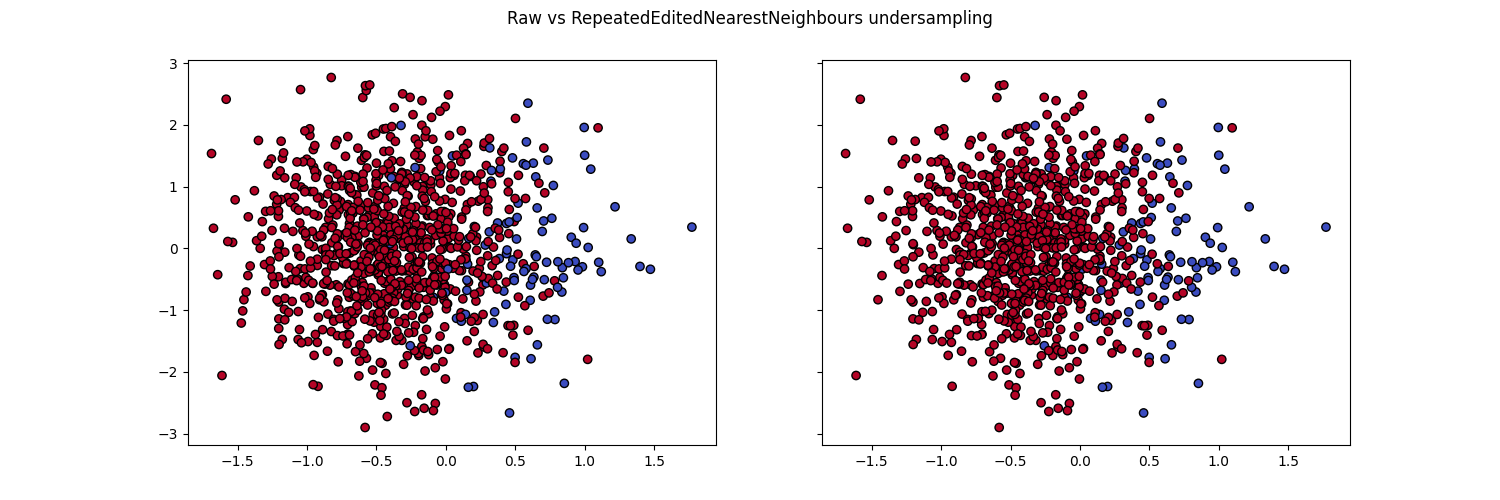
\includegraphics[width=0.6\textwidth]{images/Raw vs RepeatedEditedNearestNeighbours undersampling.png}
    \caption{RepeatedEditedNearestNeighbours örneği.}
    \label{fig:enter-label}
\end{figure}

\newpage

\subsubsection{AllKNN}
Veri setindeki her bir örnek için, k-NN algoritması kullanılarak örneğin etrafındaki komşular bulunur. Eğer bir örnek, en az k kadar komşusundan çoğunluk sınıfına aitse, bu örnek korunur. Eğer değilse, azınlık sınıfına aitse ve k değerinden az sayıda komşusu çoğunluk sınıfına aitse bu örnek veri setinden çıkarılır. Tüm örnekler bu şekilde kontrol edilerek, sınıf dengesizliği azaltmak için uygun olanlar belirlenir ve veri seti güncellenir.

\begin{lstlisting}[language=Python]
from imblearn.under_sampling import AllKNN

allk = AllKNN(sampling_strategy="auto", n_neighbors=250, kind_sel="all")
X_resampled, y_resampled = allk.fit_resample(X_train, y_train)
\end{lstlisting}

\begin{figure}[h]
    \centering
    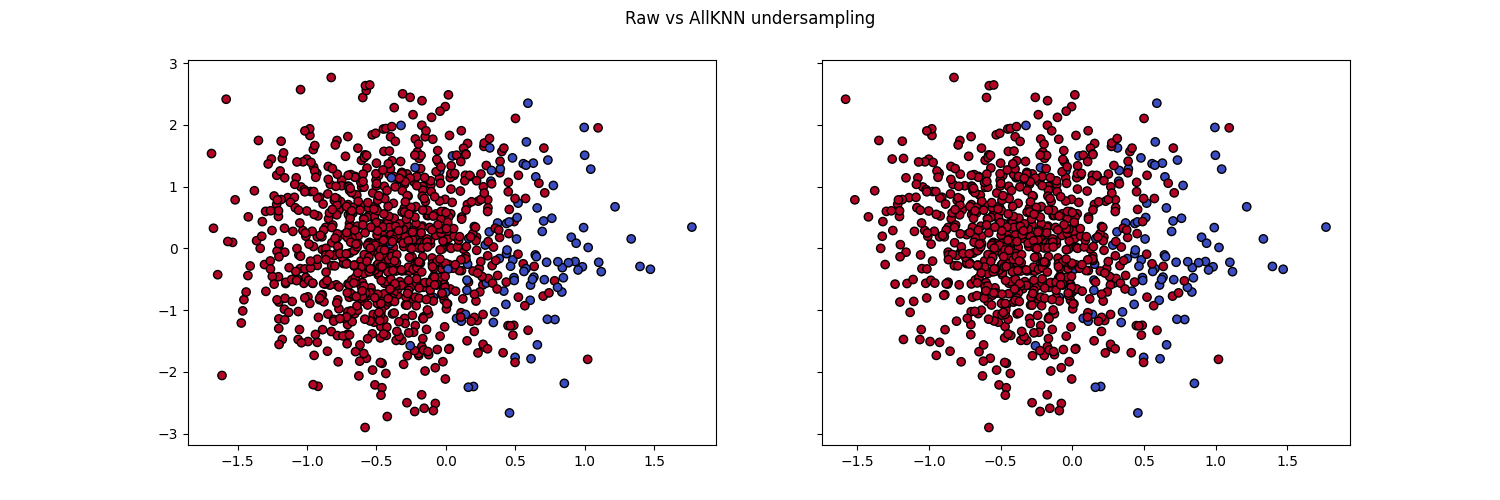
\includegraphics[width=1\textwidth]{images/Raw vs AllKNN undersampling.png}
    \caption{AllKNN örneği.}
    \label{fig:enter-label}
\end{figure}

\newpage

\subsubsection{InstanceHardnessThreshold}
Her bir örnek için, bir sınıflandırma modeli (genellikle k-NN veya bir karar ağacı kullanılır) kullanılarak örneklerin zorluk seviyesi belirlenir. Bu, örneğin yanlış sınıflandırılma olasılığı veya belirsizlik derecesi gibi faktörlere dayanabilir. Bir eşik değeri belirlenir. Bu eşik değeri, seçilecek veya kaldırılacak örneklerin zorluk seviyesini belirler. Örnekler, belirlenen eşik değerine göre değerlendirilir. Eşik değerini geçen örnekler, model için zor olan veya belirsiz olan örnekler olarak kabul edilir ve kaldırılabilir veya azaltılabilir.

\begin{lstlisting}[language=Python]
from imblearn.under_sampling import InstanceHardnessThreshold
from sklearn.linear_model import LogisticRegression

iht = InstanceHardnessThreshold(random_state=0, sampling_strategy="auto", estimator=LogisticRegression())
X_resampled, y_resampled = iht.fit_resample(X_train, y_train)
\end{lstlisting}

\begin{figure}[h]
    \centering
    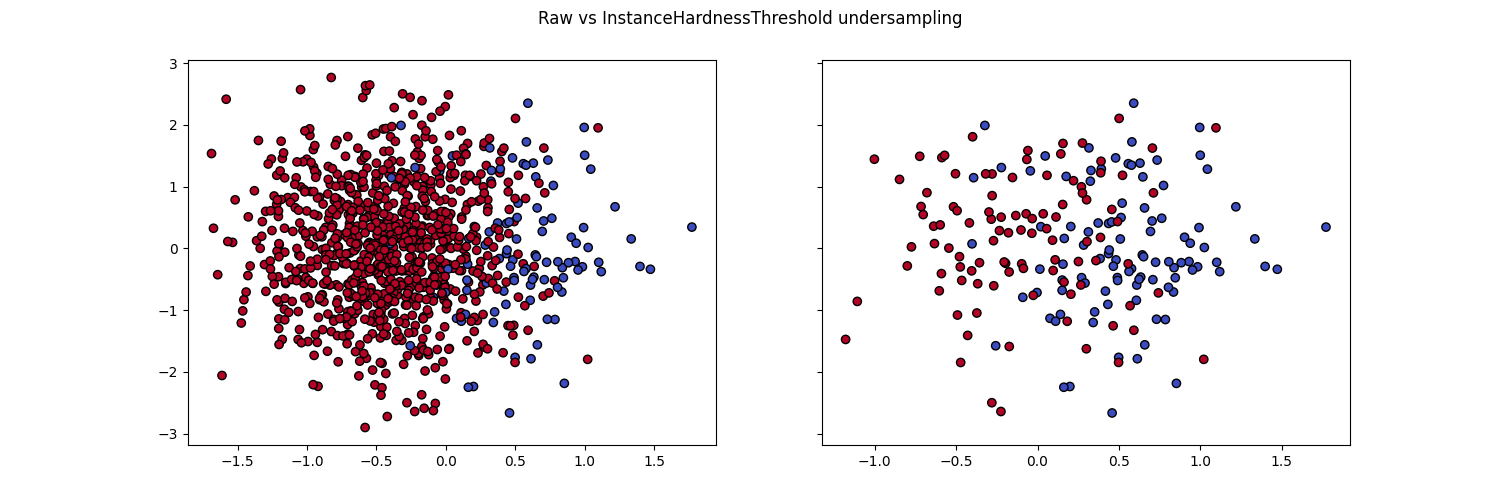
\includegraphics[width=1\textwidth]{images/Raw vs InstanceHardnessThreshold undersampling.png}
    \caption{InstanceHardnessThreshold örneği.}
    \label{fig:enter-label}
\end{figure}

\newpage